\begin{frame}[fragile]{Figure plaatsing}

    \mintinline{tex}{\begin{figure}[h]}
    \begin{center}
        \fbox{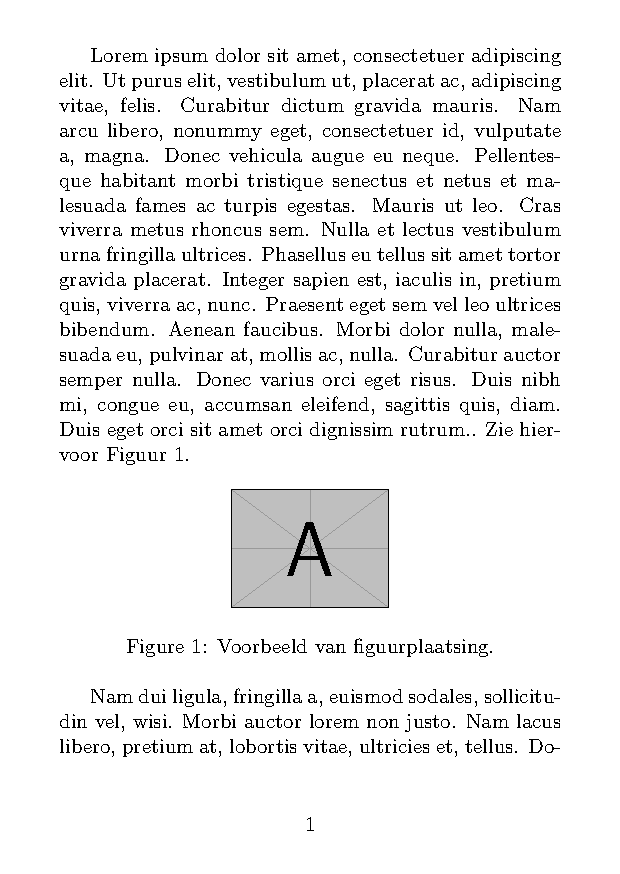
\includegraphics[page=1, height=0.70\textheight]{images/image_placement.pdf}}
        \fbox{\includegraphics[page=2, height=0.70\textheight]{images/image_placement.pdf}}
    \end{center}
\end{frame}

\begin{frame}[fragile]{Figure plaatsing}

    \mintinline{tex}{\begin{figure}[t]}
    \begin{center}
        \fbox{\includegraphics[page=3, height=0.70\textheight]{images/image_placement.pdf}}
        \fbox{\includegraphics[page=4, height=0.70\textheight]{images/image_placement.pdf}}
    \end{center}
\end{frame}

\begin{frame}[fragile]{Figure plaatsing}

    \mintinline{tex}{\begin{figure}[b]}
    \begin{center}
        \fbox{\includegraphics[page=5, height=0.70\textheight]{images/image_placement.pdf}}
        \fbox{\includegraphics[page=6, height=0.70\textheight]{images/image_placement.pdf}}
    \end{center}
\end{frame}

\begin{frame}[fragile]{Figure plaatsing}

    \mintinline{tex}{\begin{figure}[p]}
    \begin{center}
        \fbox{\includegraphics[page=7, height=0.70\textheight]{images/image_placement.pdf}}
        \fbox{\includegraphics[page=8, height=0.70\textheight]{images/image_placement.pdf}}
    \end{center}
\end{frame}


\begin{frame}[fragile]{Figure plaatsing}

    Mogelijke parameters voor figuurplaatsing: 
    \begin{itemize}[label= {\usebeamercolor[fg]{structure} \(\blacktriangleright \)}]
		\item h \textsc{(here)}: Figuur mag hier.
		\item t \textsc{(top)}: Figuur mag bovenaan een pagina.
		\item b \textsc{(bottom)}: Figuur mag onderaan een pagina.
		\item p \textsc{(page)}: Figuur mag op aparte pagina voor figuren.
		\item !\; : Override interne parameters voor floats.
		\item H \textsc{(here)}: Geen floating, altijd hier. (\mintinline{tex}{\usepackage{float}})
    \end{itemize}
    Bij meerdere letters worden verschillende opties op volgorde geprobeerd. \\
    Bijvoorbeeld: \mintinline{tex}{\begin{figure}[ht]} 

\end{frame}